\chapter{Prototype Development}
\section{Iteration overview}
This chapter presents four design iterations and methods that were used while prototyping. The table below summaries the iterations and shows what methods were used and how the prototype was evaluated.
{
\begin{table}[H]
\centering
\hskip-1.5cm\begin{tabular}{ |l|l|l|l|l| }
  \hline
  \multicolumn{5}{|c|}{Overview of iterations} \\
  \hline
\makecell[l]{Iteration} &\makecell[l]{1}
&\makecell[l]{2}
&\makecell[l]{3}
&\makecell[l]{4}\\ 
\hline
\makecell[l]{Define/Redefine} &\makecell[l]{Literature review\\ and survey}
&\makecell[l]{Redefine after\\ expert interview}
&\makecell[l]{Redefine after\\ focus group}
&\makecell[l]{Redefine after\\ SUS with experts}
\\ 
\hline
\makecell[l]{Fidelity} &\makecell[l]{Low}
&\makecell[l]{Low-mid}
&\makecell[l]{High}
&\makecell[l]{High}
\\ 
\hline
\makecell[l]{Method} &\makecell[l]{Interview with\\ experts}
&\makecell[l]{Focus group \\ design principles}
&\makecell[l]{Group survey}
&\makecell[l]{SUS with experts}\\ 
\hline
\makecell[l]{Evaluate} &\makecell[l]{Evaluate with \\ experts}
&\makecell[l]{Interview}
&\makecell[l]{SUS with experts}
&\makecell[l]{SUS with users \\heuristics with\\ experts}
\\ 
\hline
\end{tabular}
\label{Overview}
\caption{Overview of design iterations}
\end{table}
}


\section{First Iteration of Research Project}
The first design iteration started with the requirements established from the literature review and a survey conducted through social media to gather data. The survey went through two pilot studies to establish the best way to get data and was shared on Facebook. The purpose of the survey was explained in the introduction, so that the people who answered knew what they were contributing to. They were shown an example of logging exercises \ref{fig:workout log} and were explained how a likert scale works. 44 people answered the survey.
\begin{figure}[H]
    \centering
    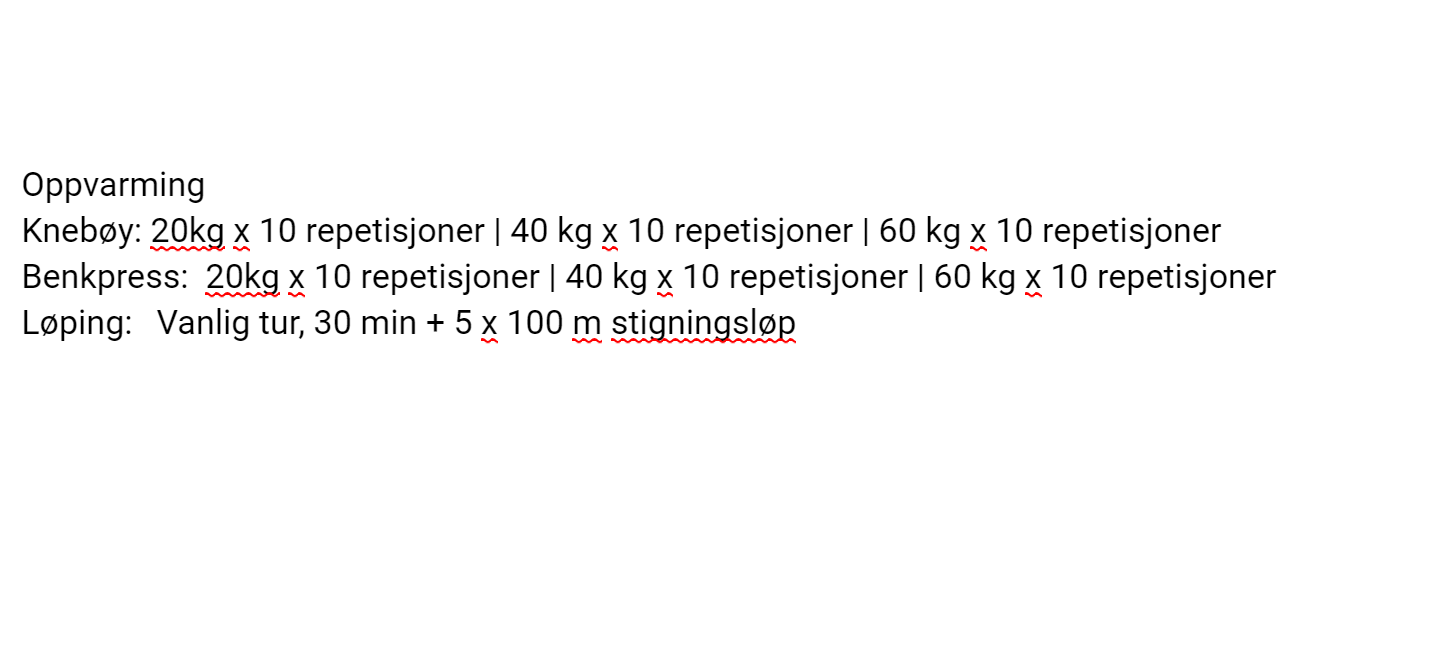
\includegraphics[width=120mm]{figures/testtest.png}
    \caption{Example of logging a workout}
    \label{fig:workout log}
\end{figure}
\subsection{The survey} \label{survey}
To establish some background information on the people that were surveyed, they were asked how often they work out and whether or not they already use an activity tracker. The majority of people that answered worked out more than 10 times a month and less than 30\% answered 5 or less.
\begin{figure}[H]%
    \centering
    {{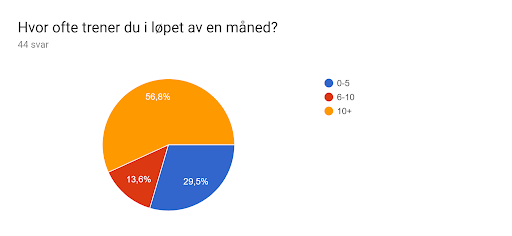
\includegraphics[width=7cm]{figures/testings.png} }}%
    \qquad
     {{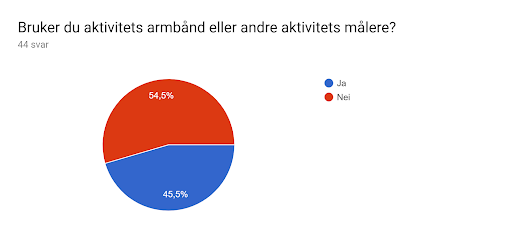
\includegraphics[width=7cm]{figures/survey2.png} }}%
    \caption{Background information}%
\end{figure}
45.5\% answered that they use an activity tracker and they were also asked to list which tracker they used which can be seen in the table below. 

\begin{table}[H]
\centering
\begin{tabular}{ |l|l| }
  \hline
  \multicolumn{2}{|c|}{Activity Tracker} \\
  \hline
Apple Watch & 2\\ 
\hline
Fenix & 1\\
\hline
Fitbit & 5\\ 
  \hline
  Garmin & 5 \\ 
  \hline
  Kadens & 1\\ 
  \hline
   Polar & 3\\ 
  \hline
   Suunto & 2\\ 
  \hline
\end{tabular}
\label{tab:3}
\caption{Survey Activity Tracker}
\end{table}

They were asked to list what kind of data they think is interesting besides logging workouts from the activity trackers and applications. Some of the answers are shown in the table below. Most people answered that knowing the heart rate, average heart rate and max heart rate is important. Also the amount of daily steps, distance of a run, amount of sleep and performance analysis were listed. 
\begin{table}[H]
\begin{tabular}{ |l|l| }
  \hline
  \multicolumn{2}{|c|}{Data from activity tracker} \\
  \hline
\makecell[l]{Norwegian} & \makecell[l]{English translation}\\ 
\hline
\makecell[l]{Distanse løpt/gått} & \makecell[l]{Distance run/walked}\\
\hline
\makecell[l]{Puls, tid og hastighet} & \makecell[l]{Heart rate, time and speed}\\ 
  \hline
\makecell[l]{Puls} & \makecell[l]{Heart rate} \\ 
  \hline
 \makecell[l]{Følge med om økten holder seg innenfor\\ mål satt før trening} & \makecell[l]{If the workout stays within the\\ pre-deterimined limits}\\ 
  \hline
  \makecell[l]{Puls, søvn, søvnforstyrrelse/urolig søvn,\\ skritt, kalorier, stigning/høydemeter} &
  \makecell[l]{Heart rate,sleep, sleep disturbances, steps,\\ calories, climb/ascent/acclivity}\\ 
  \hline
   \makecell[l]{Puls, løpedistase og tid} & \makecell[l]{Heart rate,distance run and time}\\ 
  \hline
   \makecell[l]{Skritteller,søvn og trenings analyse} &\makecell[l]{ Steps, distance, sleep and workout analysis}\\ 
  \hline
   \makecell[l]{Antall skritt gått} & \makecell[l]{Daily steps}\\ 
  \hline
   \makecell[l]{Performance, energiforbruk, treningseffekt og\\ restitusjonstid} & \makecell[l]{Performance, energy spent,\\ training effect, recovery time}\\ 
  \hline
   \makecell[l]{Gjennomsnittspuls} & \makecell[l]{Average heart rate}\\ 
  \hline
   \makecell[l]{Makspuls} & \makecell[l]{Max heart rate}\\ 
  \hline
\end{tabular}
\label{table:ActivityTrackerData}
\caption{Data from activity trackers}
\end{table}



To get more knowledge about the surveyed people`s workout habits, they were asked if they logged their workouts seen in figure \ref{workoutlogging}. The majority answered they do not log their workouts.  From the 41.9 \% of people that log their workouts were asked if they do it after or during and 70\% of them do it after they are finished with the workout.

\begin{figure}[H]
    \centering
    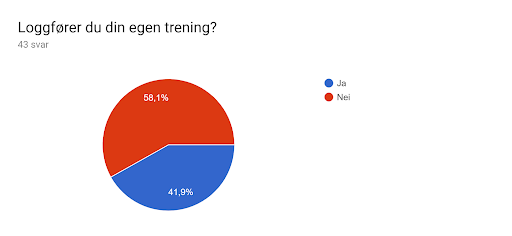
\includegraphics[width=120mm]{figures/loggforerduegentrening.png}
    \caption{Workout logging}
    \label{workoutlogging}
\end{figure}
To get an understanding of how people view others progress \ref{others}. They were asked if they feel extra motivated to workout by seeing friend`s progress, whether its strength progression or physical changes. 20 people answered that they agree or strongly agree. 13 answered neutral and 11 in total answered that they disagreed or strongly disagreed.
\begin{figure}[H]
    \centering
    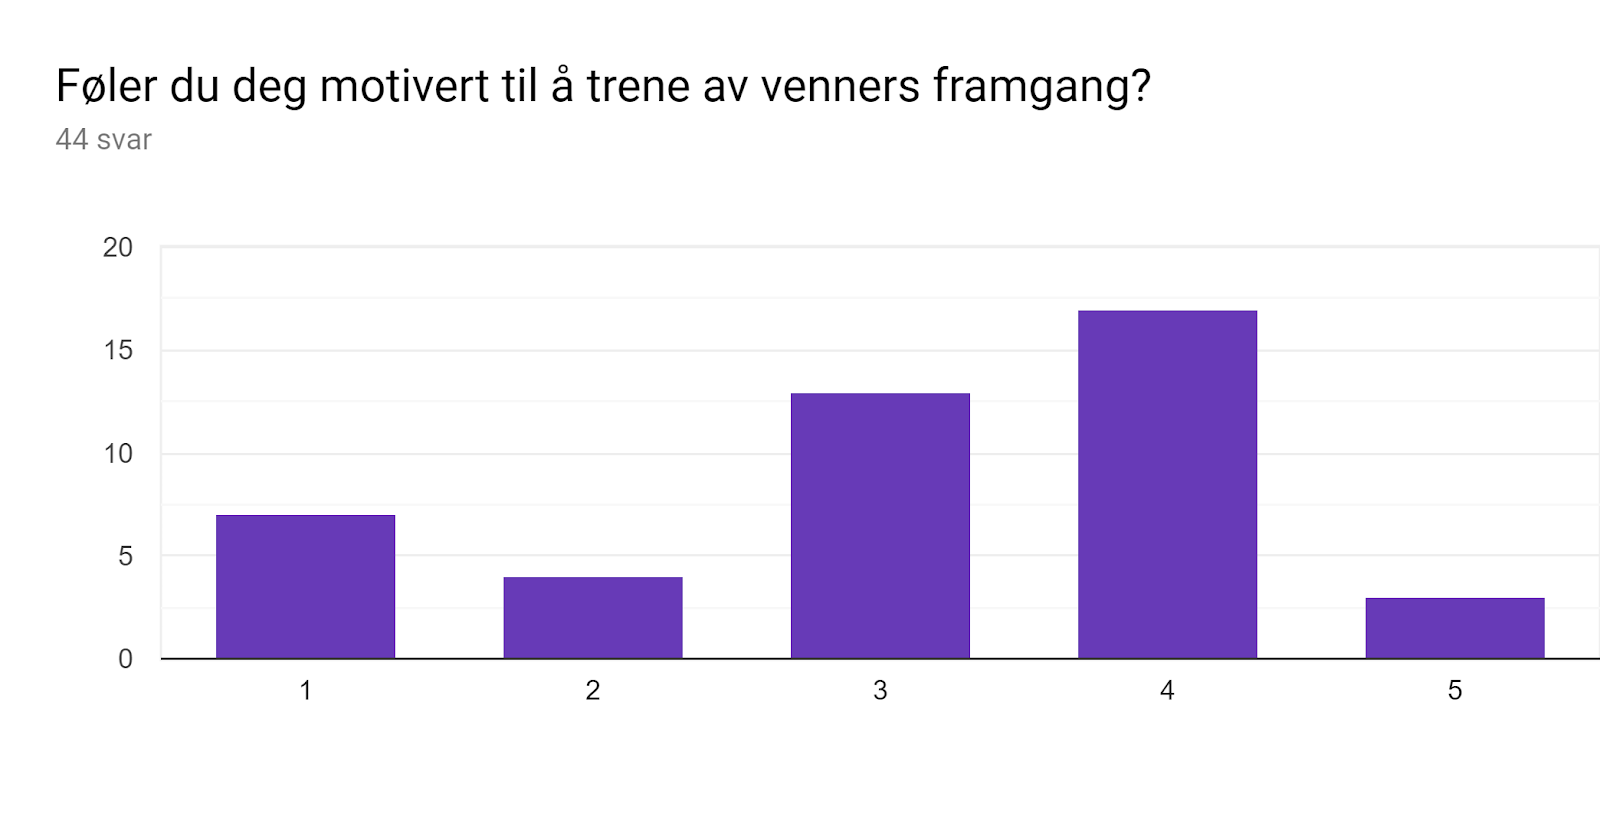
\includegraphics[width=120mm]{figures/MotivertAvAndresTrening.png}
    \caption{Motivated from others progress}
    \label{others}
\end{figure}
Since most people do not log their workouts, it is interesting to know if they would feel motivated to log their workouts if their friends could see the workout logs. However most people strongly disagree with this statement. 

\begin{figure}[H]
    \centering
    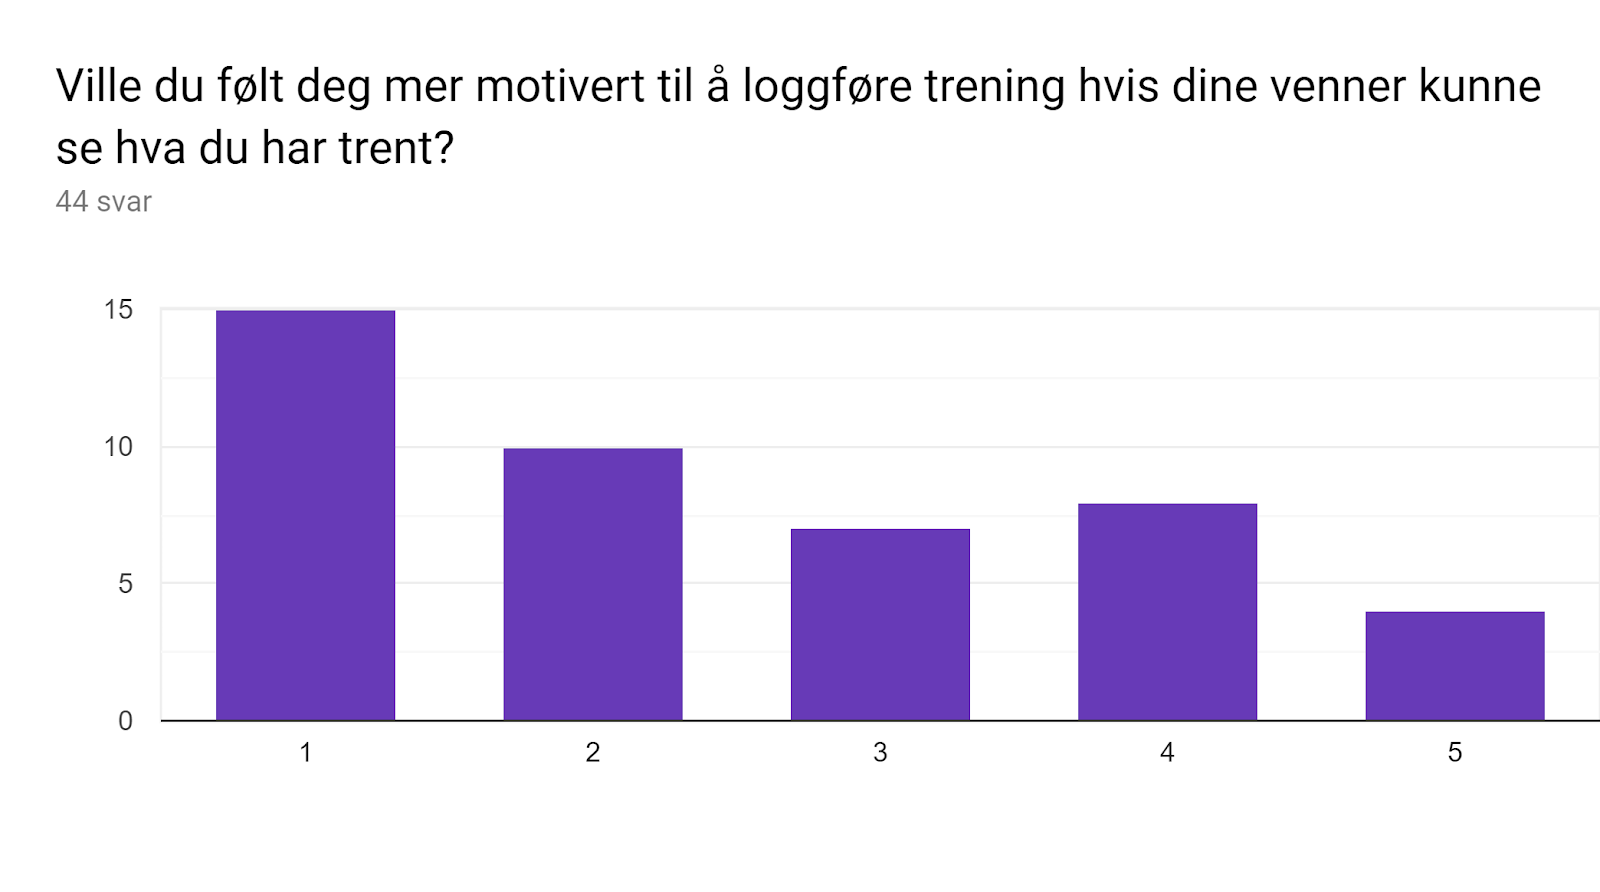
\includegraphics[width=120mm]{figures/MotivertTilLogging.png}
    \caption{Motivated to log workouts if friends could see the logs}
    \label{moti}
\end{figure}

The next question was about accountability and whether or not they would feel accountable to log their workouts if their friends could see them. The answers from figure \ref{acc} were almost identical to the motivation answers shown in figure \ref{moti} where the people mostly disagreed with the statement.

\begin{figure}[H]
    \centering
    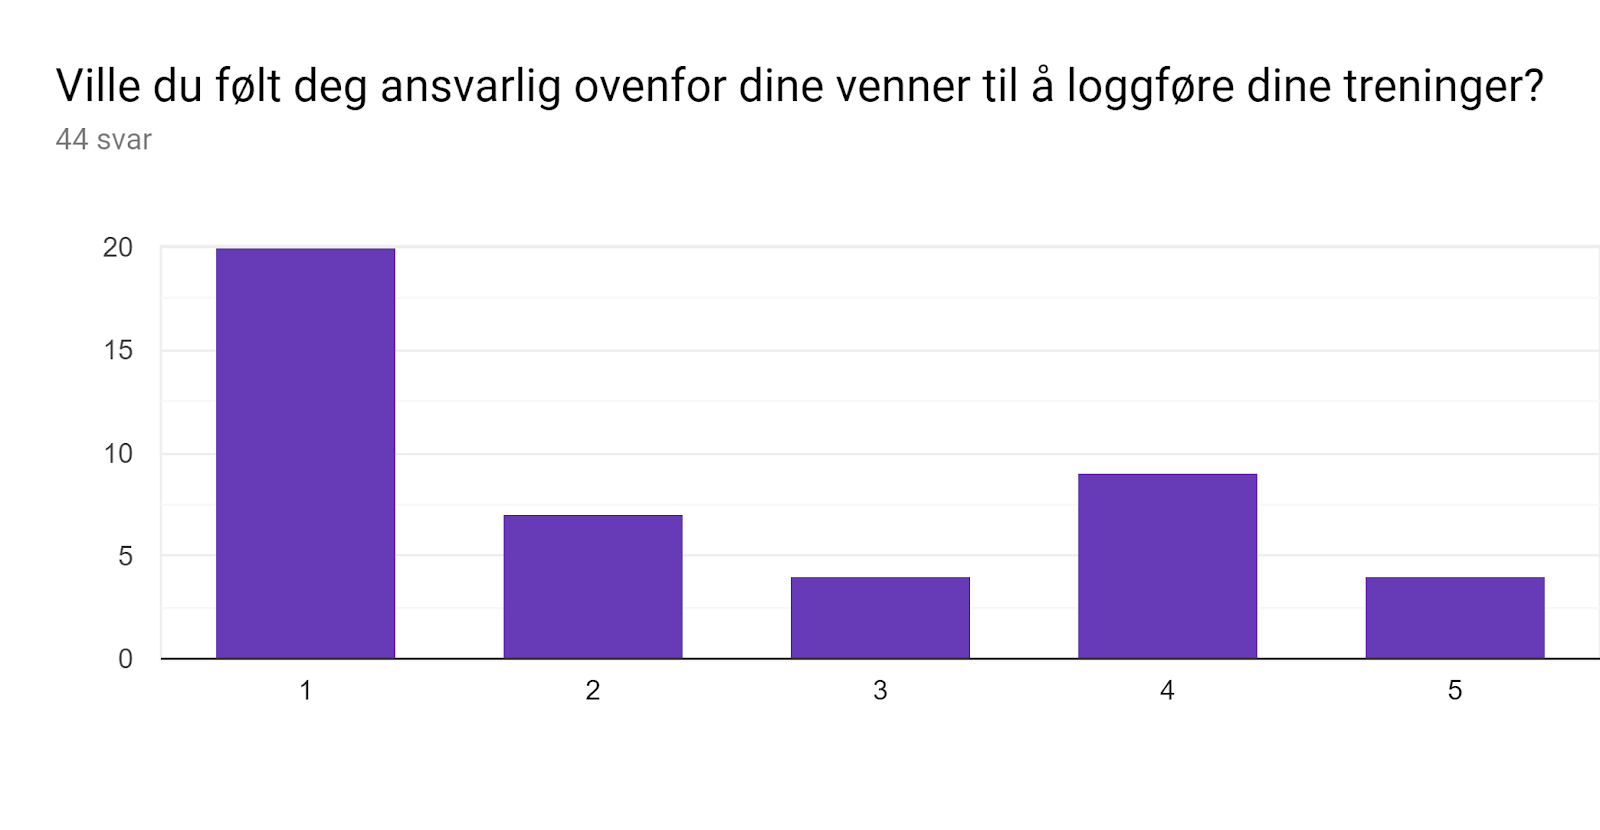
\includegraphics[width=120mm]{figures/AnsvarligLogging.png}
    \caption{Accountability from friends to log workouts}
    \label{acc}
\end{figure}
To find out if the surveyed people are interested in their friends workouts, they were asked if they were interested in friend`s progression in running, or if their friends gathered for a football game. The answers were quite mixed as shown in figure \ref{inti}, however the answers mostly disagreed with the statement. 
\begin{figure}[H]
    \centering
    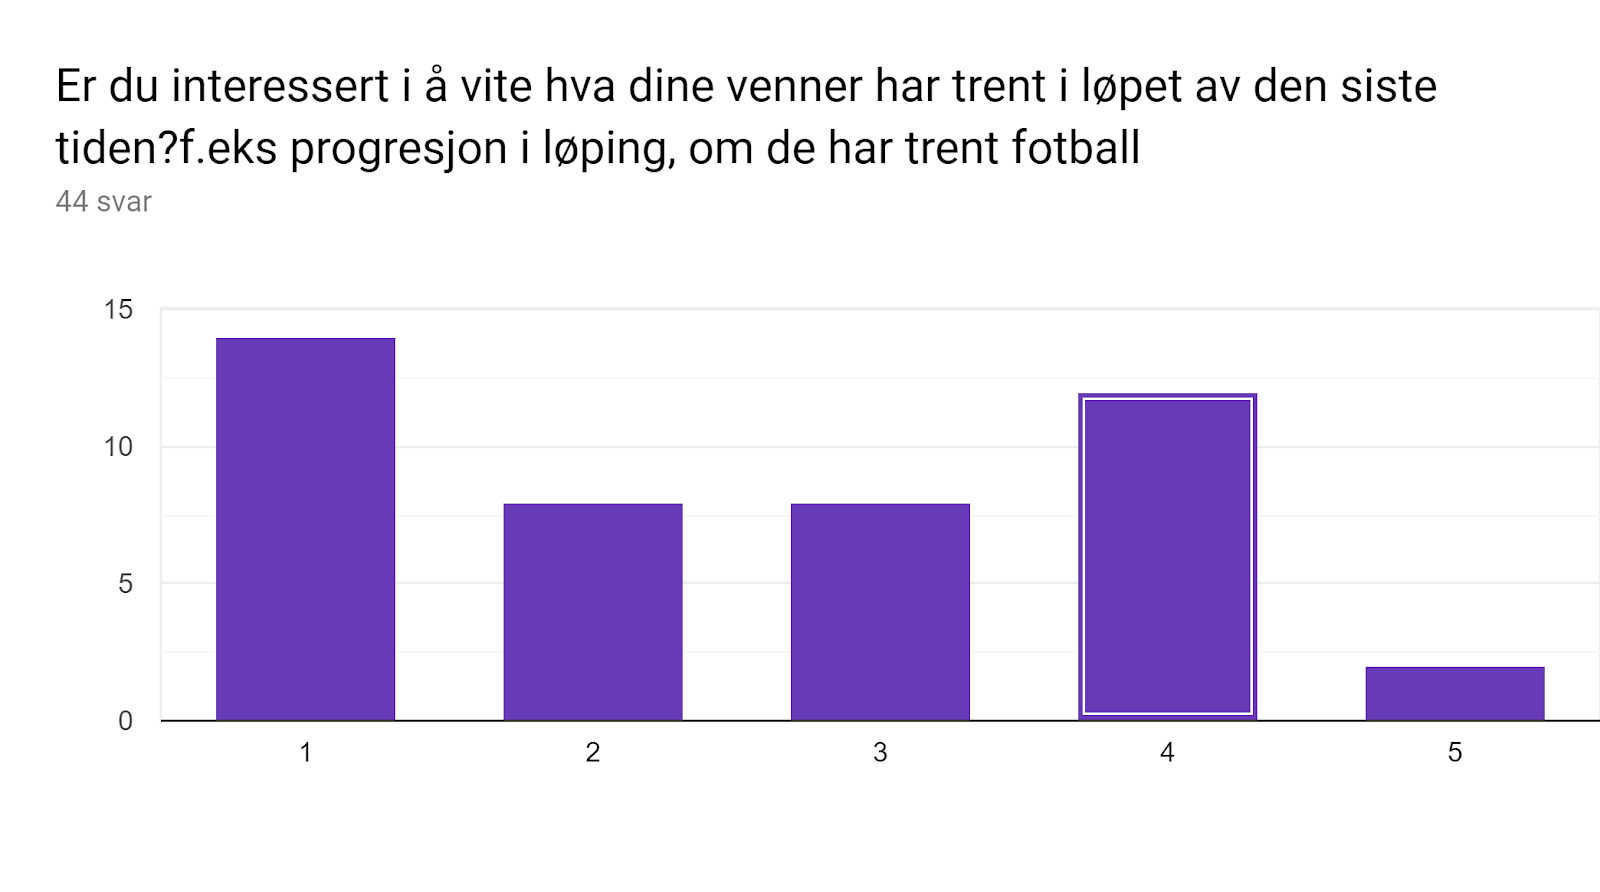
\includegraphics[width=120mm]{figures/AndresTrening.png}
    \caption{Interested in friends workouts and progress}
    \label{inti}
\end{figure}

As suggested in the literature review, having common goals is important to both stay motivated and accountable. The survey asked if it would be extra motivating to have a common workout goal that they co-operate with their friends. Examples would be running 5 kilometers together, lifting weights together or daily step challenges. The answers were mostly positive as seen in figure \ref{cgs}. Only 7 answers disagreed or strongly disagreed.
\begin{figure}[H]
    \centering
    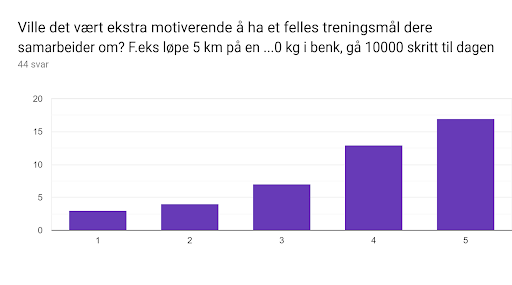
\includegraphics[width=120mm]{figures/FellesMaal.png}
    \caption{Motivation from common goals}
    \label{cgs}
\end{figure}
As a follow up to the last question, the surveyed people were asked if it is motivating to compete with friends towards a common goal. Again the answers were mostly positive to the suggestion as most people strongly agreed with the statement. 


\begin{figure}[H]
    \centering
    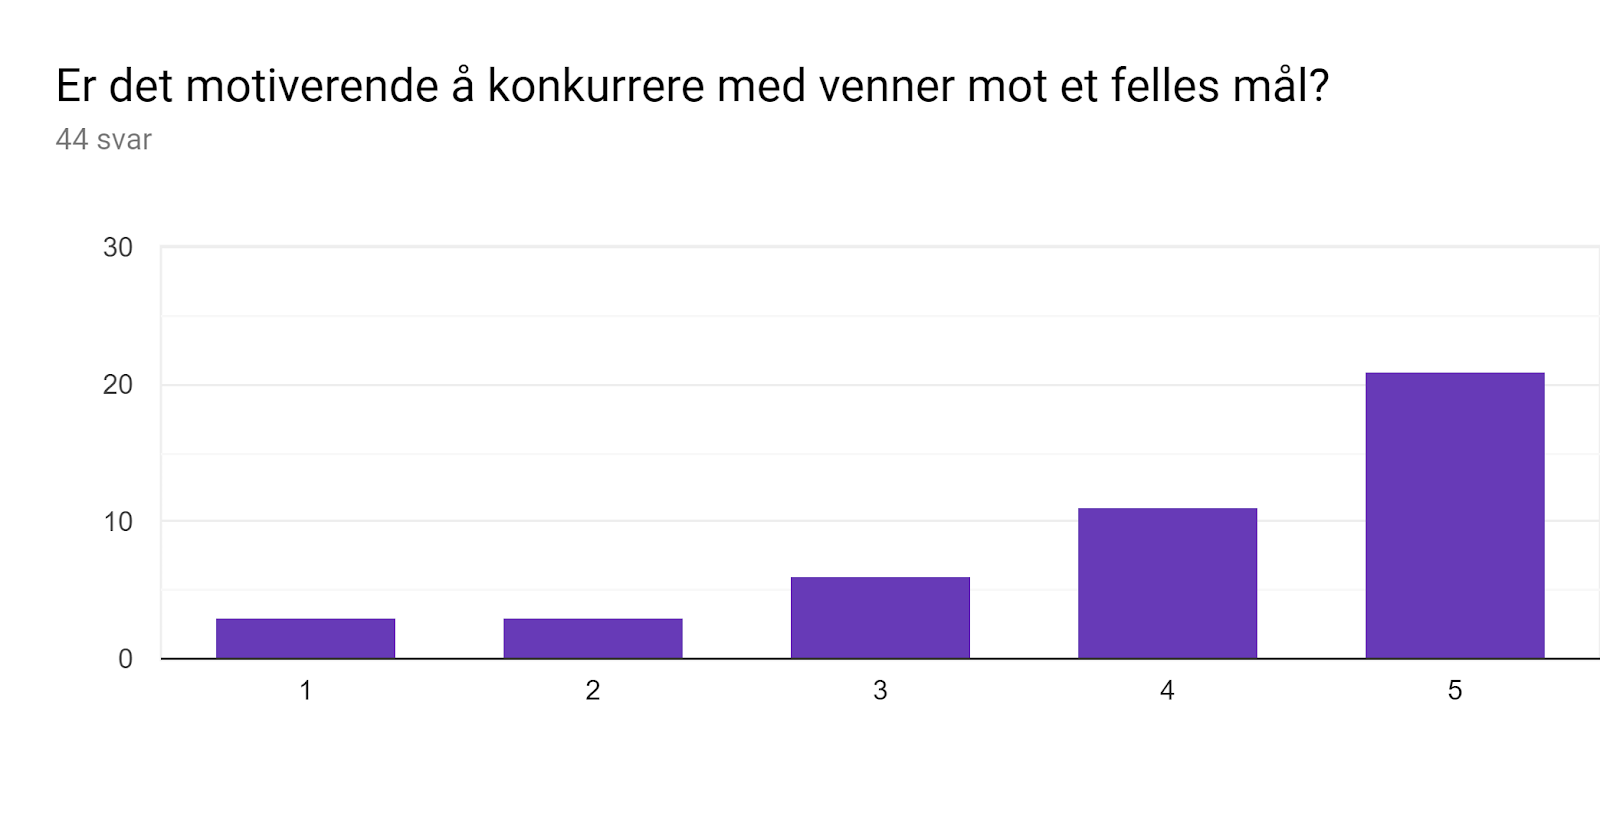
\includegraphics[width=120mm]{figures/KonkurereVenner.png}
    \caption{Competing with friends}
    \label{data}
\end{figure}
To get an idea of how members of a group would interact with each other, they were asked if they would like to get instant notifications if a member of their group was working out. The idea here is that if a member is working out at the moment, it would motivate the rest of the group to go out and do a workout.
As seen in figure \ref{instaN}, the answers are mostly strongly disagree or neutral. They prefer to have an asynchronous application instead of a synchronous application with push warnings or instant notifications.
\begin{figure}[H]
    \centering
    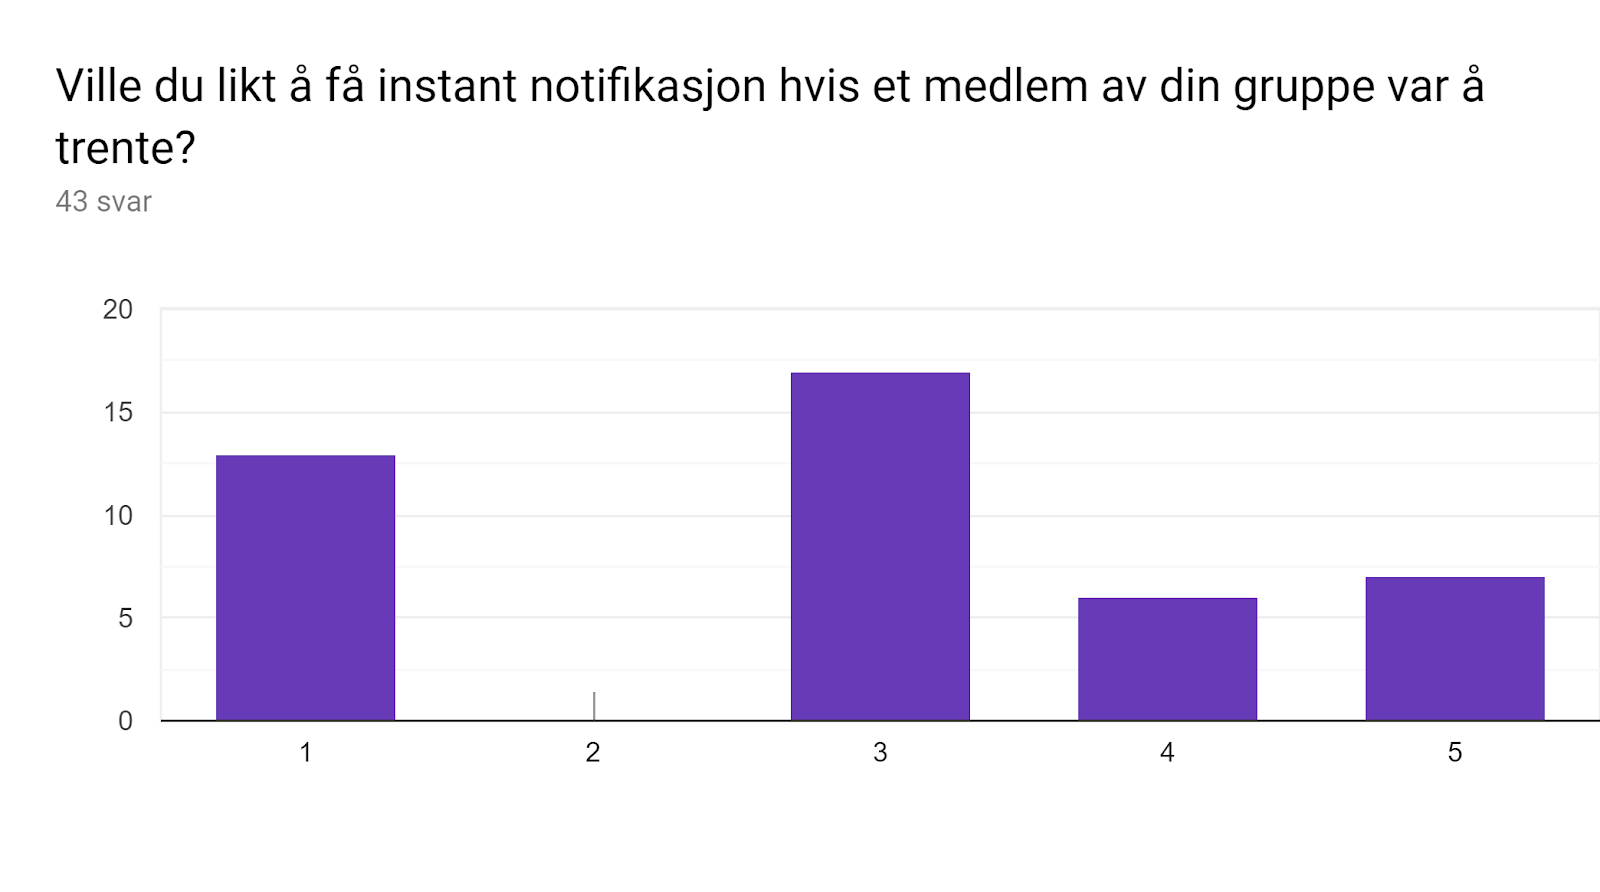
\includegraphics[width=120mm]{figures/InstantNotifikasjon.png}
    \caption{Instant notifications}
    \label{instaN}
\end{figure}

\begin{figure}[H]
    \centering
    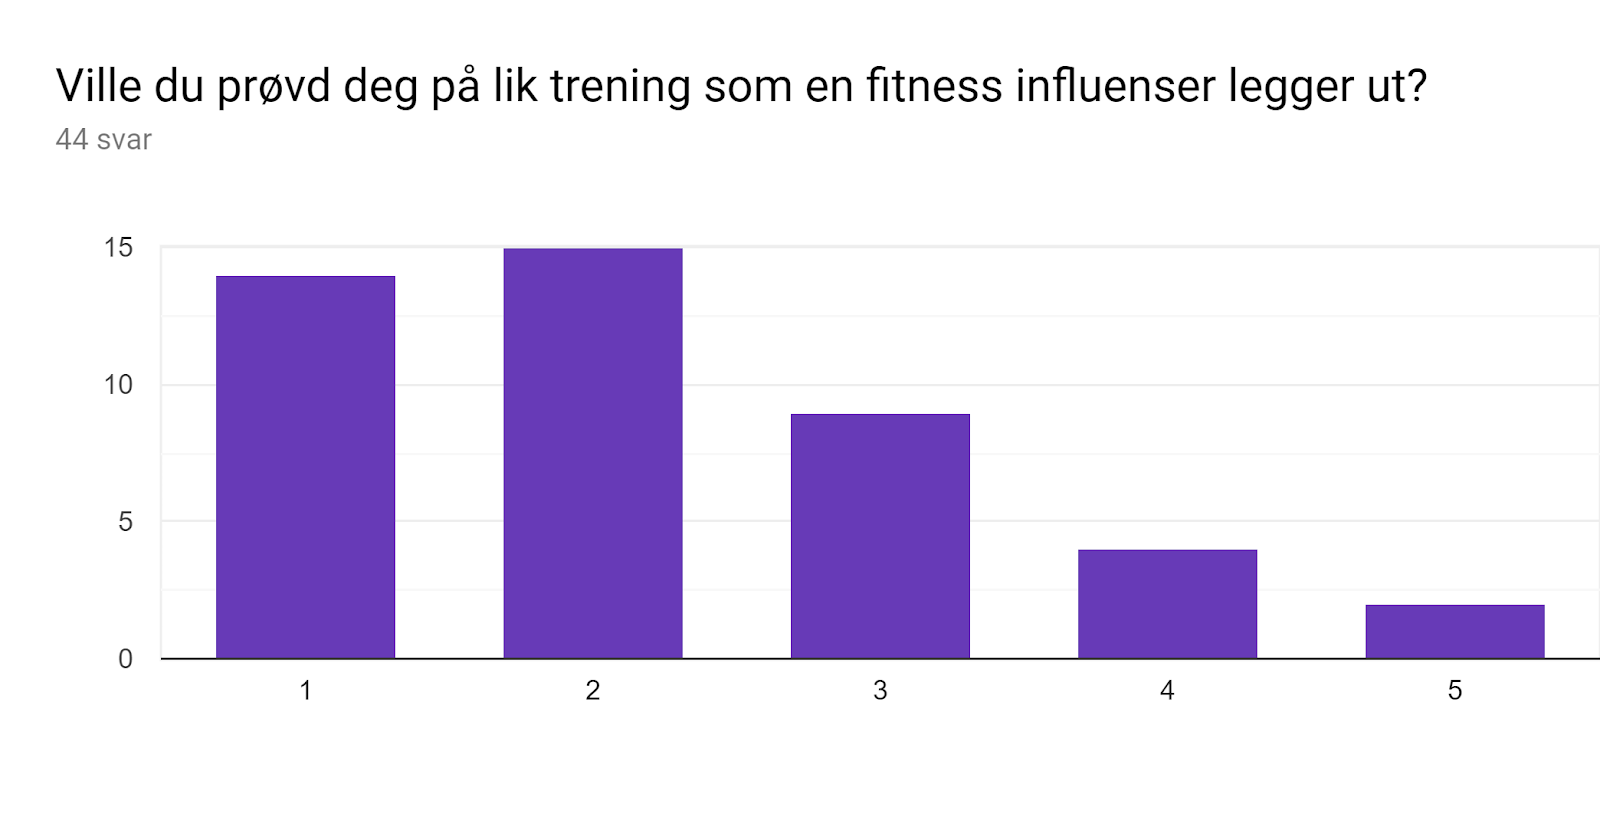
\includegraphics[width=120mm]{figures/FitnessInfluencer.png}
    \caption{Testing workouts from fitness influencers}
    \label{fitnitsinf}
\end{figure}
From the literature review it is suggested that some people take the role of a mentor and having mentors help people in the early stages by sharing information and knowledge. Fitness influencers are people that share exercises and workouts online on social media like Instagram and Snapchat. However the answers were negative and most people disagree that they would try the same workouts as fitness influencers share on social media. 
\begin{figure}[H]
    \centering
    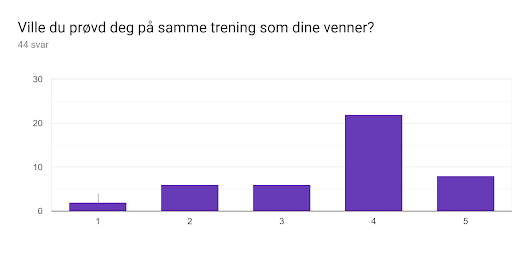
\includegraphics[width=120mm]{figures/VennerInfluencer.png}
    \caption{Testing workouts from friends}
    \label{fwork}
\end{figure}
As a follow up to figure \ref{fitnitsinf}, it is interesting to find that people much rather prefer to copy workouts from friends. Figure \ref{fwork} shows that people would like to try a workout written by a friend.
\subsection{Low-fidelity prototype}\label{lowfi}
The first version of the application was created as a sketch on paper. Several iterations were drawn on paper to test different layouts and features. The sketches were focused on the functionality of creating or joining groups and how to select and share goals. There is a workout logging feature that lets users log their own workouts and look at past workouts and a feature that lets the users look at the group members workout as well. The goals are selected by the group members and will be visible in the social group member part of the application. 
\begin{figure}[H]
    \centering
    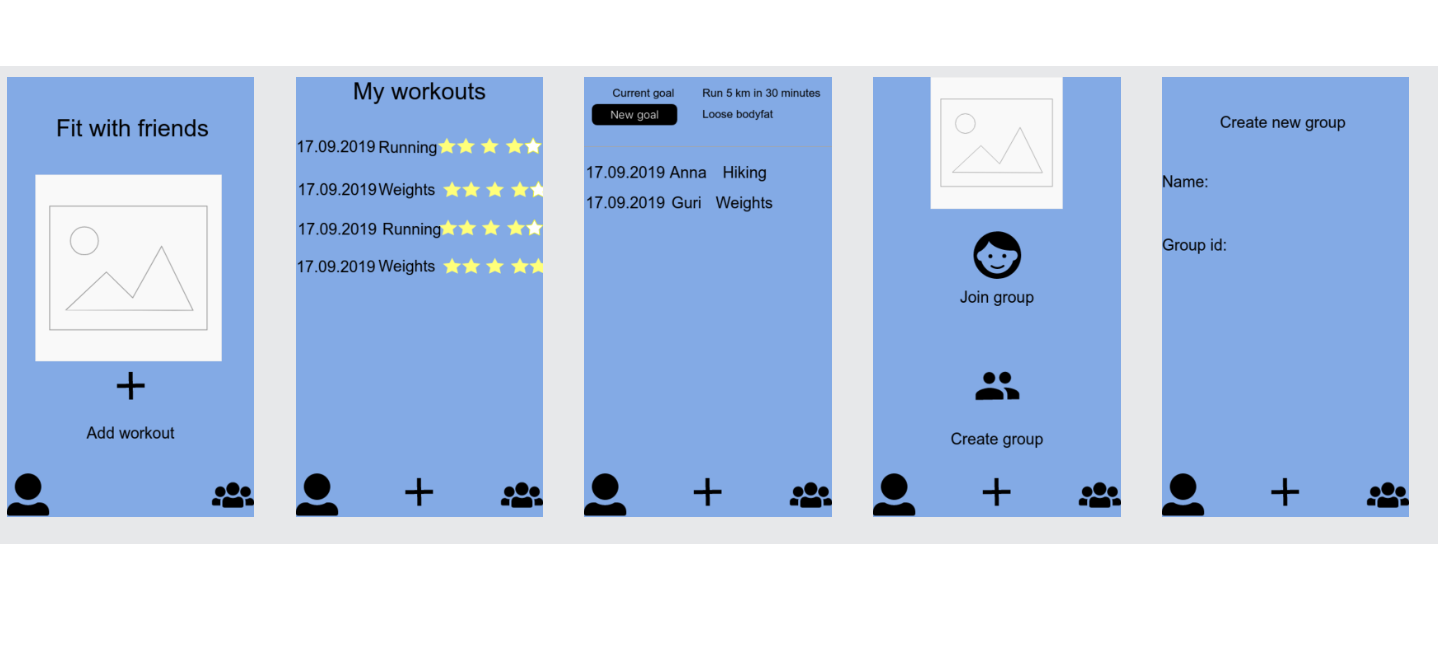
\includegraphics[width=120mm]{figures/testytestings.png}
    \caption{Wireframes for the application}
    \label{wireframe}
\end{figure}
Figure \ref{wireframe} shows some of the screens from the first wireframe that is created in the prototype program Proto.io. The bottom buttons on every screen are inspired from other social media applications. The user icon will go to your own workout log(the second screen) and the group of users will go to a group screen(the third screen) with the common goals and the other users workouts. The Add icon will be for adding workouts. The fourth and fifth screen shows the group screens, where the users will be able to join or create groups, select names for the group and then adding common goals for all their members.
\subsection{Interactive prototype}
With proto.io it is possible to add interactions and clickable buttons for the wireframes. This was used to create the first interactive low-fidelity prototype. The interactive prototype displayed the functions mentioned in section \ref{lowfi}. Instead of adding dropdown menus and clickable lists the features were presented with symbols and descriptive information to illustrate the different functions. Illustrative images were also added to improve the user experience of the low-fidelity prototype.
\begin{figure}[H]
    \centering
    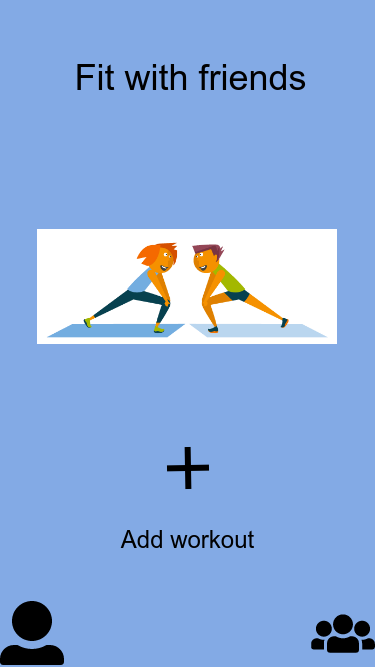
\includegraphics[scale=0.25]{figures/777.png}
    \caption{First interactive prototype with Proto.io}
    \label{intProt}
\end{figure}
\subsection{Expert interview} \label{expertinterview}
Two experts were interviewed at City Sammen, a physiotherapist and researcher and a developer, both work as personal trainers online and have worked with clients in person before. There was a brief introduction of the goals and ideas of the project, then the experts were introduced to the literature review and the answers from the survey. After a semi-structured interview was done with a set of pre-defined questions about how the personal trainers work, and the development and features of the application. 

The experts thought it was an interesting project and both agreed that setting personal goals and providing feedback and accountability is very important to keep improving the physical fitness of their clients. They also believed that having groups would increase the competition between the users and that it would keep the users accountable by "shaming" each other if they fell off.
One expert requested a way of visualising the progress towards a goal, with a progress bar or showing the progression percentage. Since it is important to show the progress that the users have made. Giving positive feedback like "great work", when a user logs their workout would be beneficial for accountability. At the end of the semi-structured interview there was a discussion between the experts about notifications. One of the experts recommended that having notifications with motivating quotes and telling the users that another user just worked out could help for the competition aspect, however the other expert agreed with the survey answers and thought that very few users would approve of this functionality. One of the experts also recommended creating the functionality in ReactJS.

\subsection{Proof of concept}
After conducting the literature review and the survey it was clear that there is a demand for group functionality for exercise applications and that it requires further research. The experts also liked the idea of an application with the proposed functionality for exercise accountability and exploring more design and technology solutions.

\section{Second Iteration of Research Project}
The second iteration consisted of changing the framework to ReactJS. This was done to test the functionality with a more realistic framework than a prototyping framework. Creating a new low-fidelity interactive prototype and implementing the current functionality there. The requirements were also redefined based on the feedback from the experts. Lastly a group of usability experts performed a SUS evaluation.
\subsection{Redefining after the expert feedback }
After the semi-structured interview with the experts some changes were made. The prototyping framework proto.io was switched with ReactJS, as an expert recommended it and it is one of the most popular frameworks for development.  The change required some learning time. 
The progress bar functionality for the group goals was also emphasized in this design iteration.

\subsection{Focus group} \label{focusgroup}
The focus group consisted three males(A,B,C) and one female(Z), who are all close friends. They were introduced to the research and were told about the ideas from the literature review. The goal of the focus group was to get the group to discuss what features and content they would like to see and most importantly stay accountable.
They were first asked if they use any fitness applications or if they have used any in the past. Two of them had used Fitbit and one had used Myfitnesspal. They had abandoned the applications because they were "boring", "not interesting" and the fun of the application quickly ended.

They were then asked if there are any features that would make them use a social fitness application.
\begin{itemize}
\item A: Having long-term goals with workout programs included, the ability to make bets with friends.
\item Z: Goals for workout frequency, general goals for working out a couple of times a week 
\item B: Competing with friends to win prizes, where the members put in money for weekly competitions. Competitions could be going to the gym the most times, working out the longest or doing the most total weight in a week. He mentioned that the application could have GPS locations for gyms, and that it should only be possible to log workouts from the gym. He also thought that having positive feedback when you log a workout is a nice touch, and the other group members should get a notification in the application when a member has logged a workout.
\item C Said that he exclusively works out alone and does not think that a social application would get him to log his workout or be interested in what his friends are doing.
\end{itemize}

The next part was dedicated to visualisation of the goals. They all agreed that the visualisation should be focused on the smaller goals, for instance having 10 workouts in total during a week for the group where every member has to contribute.  They mentioned that the bigger goals like working towards completing a marathon, or hitting a 100 kg bench press should be a personal goal and this could be visualised with a percentage bar. The intermediate objective goals could be visualised with check marks, using a green check mark for success and a orange check mark for in progress.

For the last part of the focus group the members were shown the current mid-fidelity prototype created in React. They did a walk through of the application where they could log a workout and go through the current components that had filler content.
\begin{figure}[H]
\flushright
    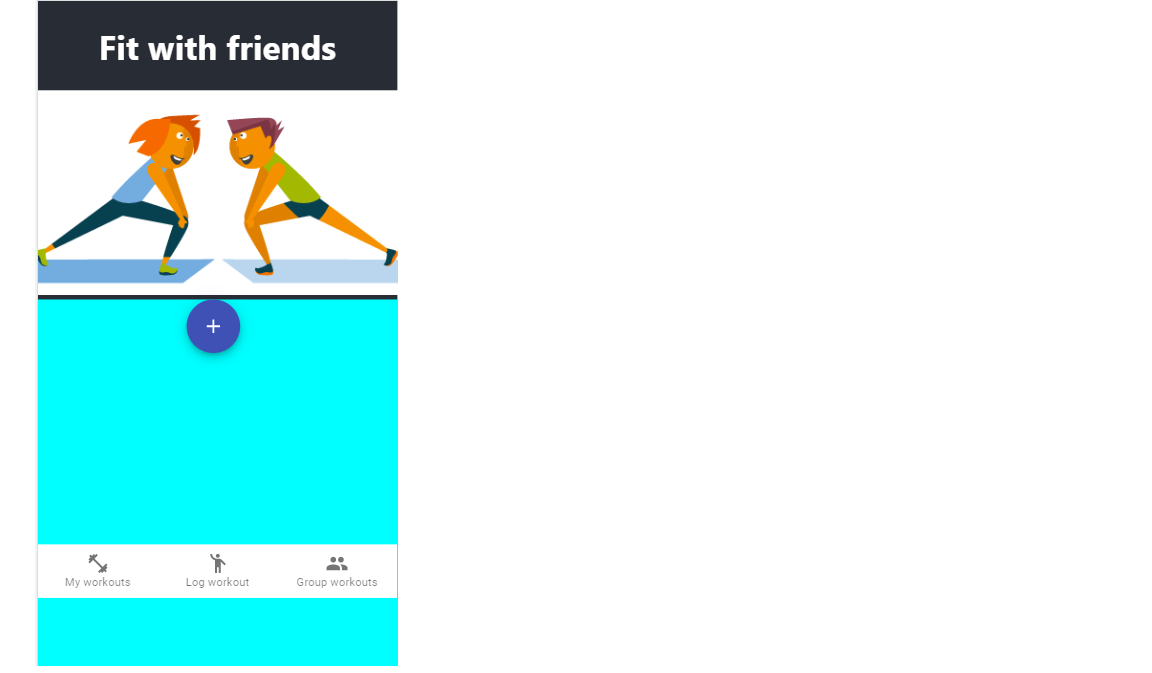
\includegraphics[scale=0.6]{figures/appenSaaLangt2.png}
    \
    \caption{Prototype shown to the focus group}
    \label{ReactProt}
\end{figure}

They were then asked about design preferences, they all agreed that having intuitive user interface and to stay social was the most important part. They thought the buttons were intuitive enough so that they understood quickly what would happen.
For the color preferences they agreed that light colors with dark text is the best option, and that it looked more professional without "aggressive screaming colors".
\subsection{Design principles}
In order to improve the prototype for testing, the five design principles were reviewed and integrated to the prototype design. For the visibility principle, text was added and replaced some of the content filler that was in "your workouts" and "your friends workouts", this added to the constraint and feedback principles as well as now it is easier to understand where in the application a user is and makes it harder to do mistakes.

For the feedback principle the navigation buttons now show a transition to the button that was pressed and the button changes colour to blue and is slightly bigger than the other two as shown in figure \ref{GruppeAss1}. The design is also consistent over every screen of the application with the same background colours, images, navigation and font. The same goes for the affordance principle as there are common icons and the layout which is inspired from social media platforms which matches the industry


\section{Third Iteration of Research Project}
For the third iteration, the feedback from the focus group was implemented to the prototype. A visualisation bar was added to the group workout to represent the personal goal of the user, and both the personal and group goals are shown as well. 
The prototype was evaluated by usability experts with SUS and a group survey.

\subsection{SUS and survey with Usability Experts} \label{susexpertos}
The evaluation of the third design iteration was conducted by six people. The usability experts were divided in to groups of three to get a feeling of the social aspect of the prototype. They were told about the previous iterations of the research project and answered a survey after doing the SUS analysis.
\begin{figure}[H]
    \flushright
    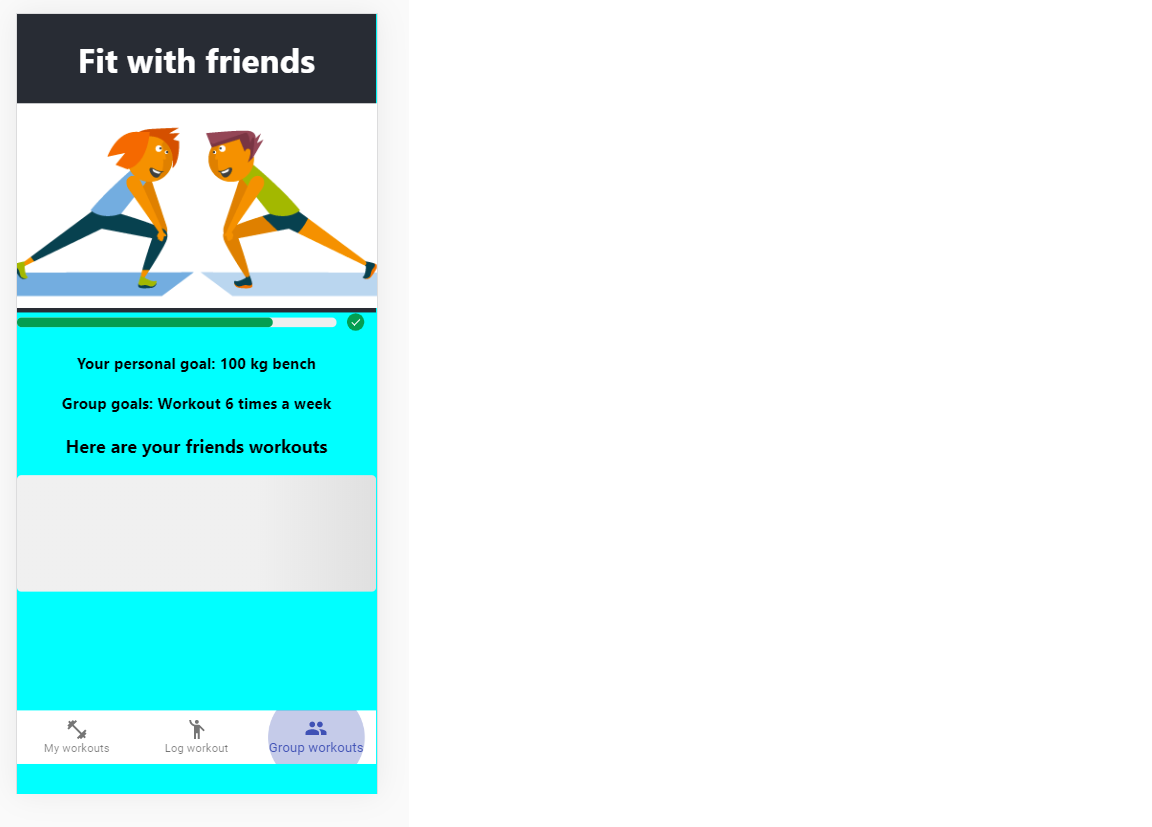
\includegraphics[scale=0.6]{figures/GruppeAspekt1.png}
    \caption{Prototype with progress bar, goals and content}
    \label{GruppeAss1}
\end{figure}

The prototype \ref{GruppeAss1} was shown to the usability experts on a laptop screen with a responsive layout window of an iPhone X. The evaluating experts consisted of six information science master students. They were guided through the prototype and explained the basic functionality of the application and how the social features would work. The experts had then a couple of minutes to click through the prototype and after they evaluated the prototype with SUS and a quick group survey.
The first group gave an average score of 90,8 and the second group gave an average score of 93,3, which is considered as best imaginable. The score might be inflated as the evaluating experts know about the SUS from beforehand and wanted to be nice.

\subsection{Group survey} \label{groupsurveyos}
Each group conducted a group survey about the functionality after completing the SUS. They were asked three questions that prompted a discussion. 
Question 1: Is there any functionality that you and your group thinks is missing?
\begin{itemize}
    \item Group 1: Would love to have a graph showing the progression towards the personal goals.
    Likes when the data is visualised, how much weight has been lifted in a gym session, how far you have run each workout and if there is progress.
    \item Group 2: Being able to log diet and share what you have eaten today, having a caloric calculator and show how many calories you have approximately used per day. One of the members pointed out that the progress bar should be below the personal goal, and the green checkmark should be changed since it looked like the goal was completed.
\end{itemize}

Question 2: Would your group be interested in having a leaderboard in the group section that would show which member is working out the most each week or month?
\begin{itemize}
    \item Group 1: Yes to both, really think both would help motivate the group members and all of them thought that it would help them to stay more active.
    \item Group 2: Yes, very motivating and would love to have a weekly rapport showing who is on top and what the members have done.
\end{itemize}

Question 3: Would you use a fitness application with the social functionality? And do you think you would continue using it for a couple of months?  ( Assuming your group of friends would too)
\begin{itemize}
    \item Group 1: Yes and "yes if I actually worked out or my friends guilted me into doing it"
    \item Group 2: Yes absolutely, especially if our friends joined.
\end{itemize}


\subsection{Redefining after feedback from usability experts}
After the feedback from the usability experts, a leaderboard was implemented to the prototype as well as a few design changes in the group section, the goal was moved above the progress bar, and the progress bar visualisation was changed so that the green checkmark only shows if the progress is complete, and the bar now is blue and shows that the goal is active.

\section{Fourth Iteration of Research Project}
The fourth iteration of the prototype consisted of testing the prototype with two users. The users evaluated the prototype with SUS and a usability test. The prototype was evaluated by experts with Nielsen`s heuristics as well.

\subsection{SUS with users} \label{suswithuseros}
A SUS evaluation was conducted by two users that contributed to the survey and the usability testing after. The users are economy students and are regular users of fitness applications.
They were shown the prototype on a laptop with iPhone X viewport and were allowed to click around to test the functionality and did three usability tasks before evaluating with SUS. Both users gave a SUS score above 90 which is seen as best imaginable and shows that the design of the prototype is intuitive and easy to use.

Additional feedback from the test users suggested adding search functionality for exercises and a calendar to easier portray the days you worked out and what you did for your workout. The results of the SUS can be seen in section \ref{susu}.

\subsection{Usability testing with users} \label{usabilitytestusers}
The participants of the usability test performed three different tasks. The tasks were performed on a laptop with iPhone X layout and were timed on every task they were given. The participants were quickly introduced to the functionality of the prototype and the research before the task, and then had some time to navigate around. The participants were presented with four different tasks that would be timed.
The users did not make any mistakes and the user interface and design seemed intuitive and easy to use. The results are shown in section \ref{usat}.

\subsection{Heuristics with experts}
Three usability experts were contacted to evaluate the prototype with Nielsen`s heuristics. The users were shown the high-fidelity prototype on a laptop with an iPhone X layout. The results are shown in section \ref{heur} .


\section{Future iterations}
After conducting the user and expert testing there were suggestions for new functionality that could be implemented in a future iteration. One suggestion was to add comments on your own workout and friends workouts to add to the social features and make it more of a social network feeling. Another suggestion which would be hard to implement was to add the data from fitness trackers to the applications or get the daily steps counter from the mobile phones of the users.  From the heuristic evaluation there are a few major usability problems that should be prioritised as well. Letting the users change their goals and adding more than one goal and adding more error prevention and easy to understand messages if an error occurs. 




